\documentclass[11pt]{article}

\usepackage[utf8]{inputenc}
\usepackage[T1]{fontenc}
\usepackage{lmodern}
\usepackage[margin=1in]{geometry}
\usepackage{amsmath}
\usepackage{amssymb}
\usepackage{booktabs}
\usepackage{multirow}
\usepackage{array}
\usepackage[table]{xcolor}
\usepackage{pgfplots}
\pgfplotsset{compat=1.18}
\usepackage{caption}
\usepackage[round]{natbib}
\usepackage{microtype}
\usepackage[colorlinks=true,linkcolor=blue!60!black,citecolor=blue!60!black,urlcolor=blue!60!black]{hyperref}
\usepackage[capitalise,noabbrev]{cleveref}

\newcommand{\ppts}{\,pp}
\newcommand{\pfam}[1]{\textsf{#1}}
\newcommand{\condn}[1]{\texttt{#1}}
\newcommand{\negA}{\cellcolor{red!12}}
\newcommand{\negB}{\cellcolor{red!25}}
\newcommand{\negC}{\cellcolor{red!40}}
\newcommand{\posA}{\cellcolor{blue!12}}
\newcommand{\posC}{\cellcolor{blue!40}}

\title{Does Perturbation Diversity Buy Robustness to Unseen Noise?\\A Family-Held-Out Study of Noisy LoRA Fine-Tuning}

\author{Soumya Ranjan Panda\\\texttt{soumyaranjanpanda.e@gmail.com}}

\date{}

\begin{document}

\maketitle

\begin{abstract}
Fine-tuning on perturbed inputs is a common way to make language models robust to noisy text, and mixing several perturbation types is often assumed to prepare a model for perturbations it has never seen. In prior work this assumption is confounded with the volume of corrupted data and with test-time exposure to the same perturbation types. We isolate it in a controlled experiment whose protocol was fixed before any test-set evaluation. Qwen2.5-0.5B-Instruct is fine-tuned with LoRA on BoolQ with half of the training questions corrupted, either by a single perturbation family or by an equal mixture of three families, and is then evaluated on three other families that never appear in training. Across two folds over six label-preserving families (18 conditions, 3 seeds, 54 training runs), the mixture does not outperform single-family training on unseen families: the pooled difference is $-0.14$\ppts{} (95\% paired-bootstrap CI $[-0.59, +0.31]$). In one fold, mixture training was 1 to 2\ppts{} less accurate on unseen families than clean fine-tuning, NEFTune, or EDA augmentation, and raising the corrupted fraction from 10\% to 100\% did not help in either fold. Robustness was strongly family-specific. Appending an irrelevant sentence to the question cost a clean-trained model 18\ppts{}, largely by biasing it towards answering ``No'', and only training data containing that perturbation closed the gap. We release code, data, run records, and per-item predictions.
\end{abstract}

\section{Introduction}

Language models deployed on real user input meet typos, odd formatting, dropped words, and irrelevant context. A natural remedy is to fine-tune on inputs that have been deliberately perturbed. Since nobody can anticipate every kind of noise, a common heuristic is to train on a \emph{diverse} mixture of perturbation types, in the hope that diversity teaches a general invariance that carries over to new kinds of noise. Mixed-type noisy instruction tuning has been reported to preserve or slightly improve accuracy under perturbed evaluation \citep{alajrami2025noisy}, and in computer vision, training on diverse augmentations improves robustness to held-out corruptions \citep{hendrycks2019benchmarking,hendrycks2020augmix}.

Two confounds make the text evidence hard to interpret. First, diversity is usually varied together with \emph{volume}: a mixture condition often contains more corrupted examples, or more corruption per example, than the single-type conditions it is compared with. Second, evaluation usually uses the \emph{same} perturbation types as training, so a benefit from mixing may only reflect that the mixture covers more of the test types. Neither design can say whether diversity itself helps with noise the model has never seen. In the six studies we examined most closely (\cref{sec:related}), none varies diversity at a fixed corruption volume, and none of the text studies evaluates on held-out perturbation families.

We test this directly. We ask: \emph{at a fixed number of corrupted training examples, does training on a mixture of perturbation families generalise better to unseen families than training on a single family?} We fine-tune Qwen2.5-0.5B-Instruct \citep{qwen2025qwen25} with LoRA \citep{hu2022lora} on BoolQ \citep{clark2019boolq}, holding the data size, the corrupted fraction (50\%), the number of optimizer steps, and all hyperparameters fixed. Six label-preserving perturbation families are split into two folds. In each fold, models train on three families and are evaluated on the other three. The protocol, including the statistical decision rule, was fixed before any test-set evaluation, and every later change is logged.

Our contributions are:
\begin{itemize}
  \item A family-held-out design that separates perturbation diversity from corruption volume and from test-time exposure, with matched clean, NEFTune \citep{jain2024neftune}, and EDA \citep{wei2019eda} baselines and a corruption-volume sweep (\cref{sec:design}).
  \item A clear null result: mixing three families gives no advantage over single-family training on unseen families in either fold (\cref{sec:primary}).
  \item Evidence that robustness from noisy fine-tuning is family-specific at this scale. Off-diagonal transfer between families is near zero or negative, and perturbed training can cost 1 to 2\ppts{} on unseen families compared with clean training (\cref{sec:secondary,sec:transfer}).
  \item An exploratory diagnosis of the one family with a large robustness gap. An appended distractor sentence mainly shifts the model's answer prior towards ``No'', and as few as 667 training examples of that family remove the shift (\cref{sec:distractor}).
\end{itemize}

\section{Related Work}
\label{sec:related}

\paragraph{Noisy instruction tuning.} \citet{alajrami2025noisy} fine-tune Qwen-2.5 and Llama-3.1 models (7B to 72B) on instructions perturbed by six operations (stop-word deletion, word shuffling, deletion, replacement, insertion, and misspelling). They sweep the perturbed fraction from 0 to 100\% at a fixed dataset size and find that tuning on perturbed instructions often preserves or slightly improves accuracy. However, every perturbed run mixes all six types, and the evaluation applies the same six types, so the contribution of diversity cannot be separated from coverage of the test types. \citet{li2026analyzing} study label, typographical, and grammatical noise in fine-tuning GPT-2, Qwen2-0.5B, and Llama-2-7B. They train each type separately and evaluate on clean test data only, and find that input noise is mild and sometimes slightly beneficial, whereas label noise is harmful. \citet{agrawal2025enhancing} compare defences against adversarial perturbations of task instructions. Their trained defences use a mixture of attacks that includes the test attacks.

\paragraph{Embedding noise and contextual distractors.} NEFTune \citep{jain2024neftune} adds uniform noise to input embeddings during instruction tuning and improves open-ended answer quality. It introduces no discrete text noise and was not evaluated for robustness to perturbed inputs, which makes it a useful control here. RAFT \citep{zhang2024raft} trains retrieval-augmented models with irrelevant distractor documents and shows robustness to the number of test-time documents. That is a shift within a single noise family.

\paragraph{Transfer between perturbation types.} In vision, \citet{kang2019transfer} measure a full train-type by test-type grid for adversarial training and find that robustness often fails to transfer between types and can even hurt. \citet{tramer2019adversarial} study adversarial training against several perturbation types at once. \citet{hendrycks2019benchmarking} established evaluation on held-out common corruptions, and AugMix \citep{hendrycks2020augmix} showed that mixing diverse augmentations improves robustness to such corruptions. In NLP, \citet{belinkov2018synthetic} showed that character-level machine translation models break under synthetic and natural noise, and that training on one kind of noise does not reliably confer robustness to other kinds.

To our knowledge, no prior text study varies perturbation diversity at a fixed corruption volume while testing on held-out perturbation families. The vision transfer results give a prior reason to expect a null result, which makes the question worth testing directly rather than assuming.

\section{Experimental Design}
\label{sec:design}

\subsection{Task, model, and data}

We use BoolQ \citep{clark2019boolq}, a reading-comprehension task where each item is a passage, a yes/no question, and a binary answer. Short, exactly scorable answers make accuracy unambiguous. We take the first 6{,}000 items of the BoolQ training split, in dataset order, and partition them into 4{,}000 training, 500 validation, 500 development, and 1{,}000 test items. The gold answer is ``Yes'' for 63.4\% of test items. The base model is Qwen2.5-0.5B-Instruct \citep{qwen2025qwen25}, prompted with a fixed system instruction to answer only ``Yes'' or ``No'' to a \emph{Passage}/\emph{Question} pair in the model's chat template.

\subsection{Perturbation families}

We use six label-preserving perturbation families, applied to the \emph{question} only. The passage is never perturbed. \Cref{tab:families} lists them with their parameters and the share of test questions each one actually changes. All perturbations are deterministic given a per-item seed. Training and test perturbations use disjoint seed ranges, and test perturbations are generated only from test items.

\begin{table}[t]
\centering
\small
\caption{Perturbation families. ``Changed'' is the share of the 1{,}000 test questions altered by the perturbation (a short question can be left unchanged by a probabilistic edit). Examples are perturbed versions of real test questions.}
\label{tab:families}
\begin{tabular}{@{}l p{4.6cm} r p{5.2cm}@{}}
\toprule
Family & Operation & Changed & Example output \\
\midrule
\pfam{typo} & per letter with $p{=}0.05$: swap with neighbour, keyboard-adjacent substitution, or deletion & 80.0\% & \emph{is the vampire diaries related to the originalz} \\
\pfam{formatting} & random upper/lower/alternating case, punctuation removal or duplication, extra spaces & 98.1\% & \emph{was MoSt of the CiViL war fought ON confederate soil} \\
\pfam{deletion} & drop each word with $p{=}0.15$ (keep at least 3 words) & 77.5\% & \emph{was most of the civil war fought confederate soil} \\
\pfam{shuffle} & swap adjacent words with $p{=}0.2$ (no chained swaps) & 82.3\% & \emph{was most of the civil war fought confederate on soil} \\
\pfam{distractor} & append one of 8 fluent, true, irrelevant sentences & 100.0\% & \emph{\ldots{} confederate soil Jupiter has the shortest day of all the planets in the solar system.} \\
\pfam{synonym} & replace content words with $p{=}0.3$ by a WordNet \citep{miller1995wordnet} lemma & 79.7\% & \emph{was most of the civil war fought on confederate dirty} \\
\bottomrule
\end{tabular}
\end{table}

\subsection{Folds and conditions}

The six families form two folds with full family-level holdout. In \textbf{fold A}, models train on \pfam{typo}, \pfam{formatting}, and \pfam{deletion}, and the unseen families are \pfam{shuffle}, \pfam{distractor}, and \pfam{synonym}. \textbf{Fold B} is the exact reverse. Every training set has exactly 4{,}000 examples, and the corrupted examples are always perturbed copies of the same 2{,}000 training questions (items 2{,}001 to 4{,}000). The conditions are:

\begin{itemize}
  \item \condn{single\_<family>} (3 per fold): 2{,}000 clean examples and 2{,}000 examples corrupted by one seen family (50\% corruption).
  \item \condn{mixed3\_f0.50} (primary, 1 per fold): 2{,}000 clean examples and 2{,}000 corrupted examples split evenly across the three seen families (667, 667, 666).
  \item \condn{mixed3} volume sweep (3 per fold): corrupted fraction 0.10, 0.25, and 1.00, built the same way.
  \item \condn{augment} (1 per fold): an EDA baseline \citep{wei2019eda} with 2{,}000 clean and 2{,}000 augmented examples. It uses only EDA operations that do not overlap the fold's unseen families: random deletion and insertion for fold A, and random swap, insertion, and synonym replacement for fold B.
  \item Shared across folds: \condn{clean} (0\% corruption) and \condn{neftune} (clean data with NEFTune, $\alpha{=}5$).
\end{itemize}

This gives 18 conditions. Each is trained with seeds 0, 1, and 2, which control LoRA initialisation, dropout, and data order (the perturbed data is fixed). Together with one evaluation of the untuned model, the study has 55 runs.

\subsection{Training and evaluation}

All conditions use identical hyperparameters (\cref{tab:hparams} in \cref{app:details}): LoRA with $r{=}16$, $\alpha{=}32$, and dropout 0.05 on all attention and MLP projections (8.8M trainable parameters, 1.75\% of the model), and AdamW with learning rate $2\times10^{-4}$, 3\% warmup, and cosine decay. Training runs for 2 epochs at an effective batch size of 16, giving exactly 500 optimizer steps in every condition. The loss is computed on the answer token and end-of-turn token only. Sequences are capped at 512 tokens by truncating the passage, never the question (15 of 4{,}000 training items). Training used fp16 mixed precision on a single NVIDIA T4. A run took on average 33 minutes of training and 10 minutes of evaluation, about 38 GPU-hours in total.

Each trained model is evaluated exactly once on the 1{,}000-item test set in seven versions: clean and one per family. All seven versions perturb the same questions in the same order. We score a single forward pass and compare the logits of the ``Yes'' and ``No'' tokens. The prediction is ``Yes'' if $p(\text{Yes}) > 0.5$ after renormalising over the two tokens. This avoids parsing generated text and gives per-item probabilities for paired statistics. The final model after 500 steps is evaluated, with no checkpoint selection, and no hyperparameters were tuned.

\subsection{Statistical analysis}

For fold $f$, the primary effect is
\begin{equation}
\Delta_f = \operatorname{acc}_{U_f}(\text{Mixed-3}) - \tfrac{1}{3}\textstyle\sum_{k=1}^{3} \operatorname{acc}_{U_f}(\text{single}_k),
\end{equation}
where $\operatorname{acc}_{U_f}$ is accuracy averaged over the fold's three unseen families $U_f$ and over seeds. The pooled effect averages $\Delta_A$ and $\Delta_B$. We compute a per-item difference (averaged over families and seeds) and form a 95\% percentile confidence interval from 10{,}000 paired bootstrap resamples of the 1{,}000 test questions \citep{efron1993bootstrap}. Because all test versions share the same questions, one resample of question indices is applied jointly to every family, seed, and condition. This interval reflects uncertainty from the test items, not from training randomness. The protocol therefore declares an effect \emph{meaningful} only if (i) the CI excludes zero \emph{and} (ii) $|\Delta|$ exceeds the standard deviation of the effect across the three seeds. Secondary contrasts use the same procedure and are not corrected for multiple comparisons. The volume sweep is reported descriptively.

\subsection{Protocol and deviations}

The question, design, model, hyperparameters, splits, and decision rule were fixed before any test-set evaluation. Six implementation decisions were logged before any test result was seen. They are summarised in \cref{app:deviations}. The most consequential is that the NEFTune baseline is shared across folds (it does not depend on the fold), which gives 54 rather than 57 training runs.

\section{Results}
\label{sec:results}

All 55 runs completed. Three runs were executed twice after interrupted cloud sessions, and both executions produced identical accuracies on every evaluation set, which confirms that training and evaluation are deterministic given the seed. The analysis was run twice, in the cloud and locally, with identical output. Accuracy for every condition and test set is given in \cref{tab:full} (\cref{app:full}).

\subsection{Primary result: no benefit from diversity}
\label{sec:primary}

\begin{table}[t]
\centering
\small
\caption{Primary comparison on the fold's \emph{unseen} families: Mixed-3 at 50\% corruption minus the mean of the three single-family models. Accuracies in \%. Effects in percentage points with 95\% paired-bootstrap CIs. ``Seed SD'' is the standard deviation of the effect across seeds.}
\label{tab:primary}
\begin{tabular}{@{}lccccc l@{}}
\toprule
Fold (unseen families) & Mixed-3 & Mean single & $\Delta$ & 95\% CI & Seed SD & Verdict \\
\midrule
A (\pfam{shuffle}, \pfam{distractor}, \pfam{synonym}) & 69.06 & 69.76 & $-0.71$ & $[-1.38, -0.05]$ & 1.11 & not meaningful \\
B (\pfam{typo}, \pfam{formatting}, \pfam{deletion}) & 77.18 & 76.76 & $+0.42$ & $[-0.24, +1.08]$ & 0.48 & null \\
Pooled & 73.12 & 73.26 & $-0.14$ & $[-0.59, +0.31]$ & 0.38 & null \\
\bottomrule
\end{tabular}
\end{table}

\Cref{tab:primary} gives the primary result. Training on a mixture of three families did not improve accuracy on unseen families in either fold. In fold B the effect is small and its CI includes zero. In fold A the point estimate is negative, and its CI just excludes zero, but the effect is smaller than its own variation across seeds, so by the pre-specified rule it is not meaningful. The per-seed effects change sign in both folds (fold A: $-1.17$, $-1.51$, $+0.56$; fold B: $+0.88$, $+0.47$, $-0.08$). The pooled CI rules out a benefit larger than about $0.3$\ppts{}.

\subsection{Secondary contrasts}
\label{sec:secondary}

\begin{table}[t]
\centering
\small
\caption{Secondary contrasts: Mixed-3 at 50\% minus the named condition, in percentage points. ``Test'' indicates which test versions are averaged. \textbf{Bold}: meaningful under the protocol rule. These 14 contrasts are not corrected for multiplicity.}
\label{tab:secondary}
\begin{tabular}{@{}llrcrl@{}}
\toprule
Comparison & Test & $\Delta$ & 95\% CI & Seed SD & Verdict \\
\midrule
\multicolumn{6}{@{}l}{\emph{Fold A}} \\
clean baseline & unseen & $\mathbf{-2.29}$ & $[-3.14, -1.48]$ & 1.03 & meaningful \\
NEFTune & unseen & $\mathbf{-2.06}$ & $[-2.92, -1.17]$ & 0.20 & meaningful \\
EDA augmentation & unseen & $\mathbf{-1.24}$ & $[-2.07, -0.40]$ & 0.50 & meaningful \\
best single (\pfam{formatting}) & unseen & $-1.01$ & $[-1.78, -0.27]$ & 1.48 & not meaningful \\
mean single & seen & $-0.32$ & $[-1.00, +0.35]$ & 1.00 & null \\
mean single & clean & $-0.74$ & $[-1.63, +0.12]$ & 0.62 & null \\
clean baseline & clean & $-0.57$ & $[-1.70, +0.53]$ & 0.47 & null \\
\midrule
\multicolumn{6}{@{}l}{\emph{Fold B}} \\
clean baseline & unseen & $+0.37$ & $[-0.43, +1.17]$ & 0.57 & null \\
NEFTune & unseen & $+0.06$ & $[-0.77, +0.88]$ & 0.78 & null \\
EDA augmentation & unseen & $-0.32$ & $[-1.11, +0.48]$ & 0.58 & null \\
best single (\pfam{distractor}) & unseen & $+0.20$ & $[-0.54, +0.96]$ & 0.60 & null \\
mean single & seen & $\mathbf{+4.51}$ & $[+3.61, +5.40]$ & 0.88 & meaningful \\
mean single & clean & $+0.83$ & $[-0.02, +1.67]$ & 0.62 & null \\
clean baseline & clean & $+0.70$ & $[-0.37, +1.77]$ & 1.21 & null \\
\bottomrule
\end{tabular}
\end{table}

\Cref{tab:secondary} compares Mixed-3 with the baselines. Two patterns stand out.

\paragraph{Fold A: perturbed training costs a little on unseen families.} On fold A's unseen families, Mixed-3 is meaningfully less accurate than the clean baseline ($-2.29$\ppts{}), NEFTune ($-2.06$\ppts{}), and EDA augmentation ($-1.24$\ppts{}). On the clean test set it is indistinguishable from the clean baseline ($-0.57$\ppts{}, null), so the cost is specific to perturbed inputs. The drop relative to clean training appears in all three unseen families (\pfam{shuffle} 76.3 vs.\ 78.1, \pfam{distractor} 57.5 vs.\ 60.8, \pfam{synonym} 73.3 vs.\ 75.1), and all three fold A single-family models also fall below the clean baseline on these families (\cref{tab:transfer}). In fold B, Mixed-3 is indistinguishable from every baseline.

\paragraph{Fold B's seen-family gain is a design artefact.} Mixed-3 beats the mean single-family model on fold B's \emph{seen} families by $+4.51$\ppts{}. This does not indicate a benefit of diversity. Only one of fold B's three single-family models trains on \pfam{distractor}, the one family where training produces a large gain (\cref{sec:transfer}). The other two score near 60\% on it, which pulls down the single-family mean. Mixed-3 contains \pfam{distractor} examples, so it does not have this gap. On fold A's seen families, where no family has a large gap, the corresponding contrast is null ($-0.32$\ppts{}).

\subsection{Corruption volume does not help either}
\label{sec:sweep}

\begin{figure}[t]
\centering
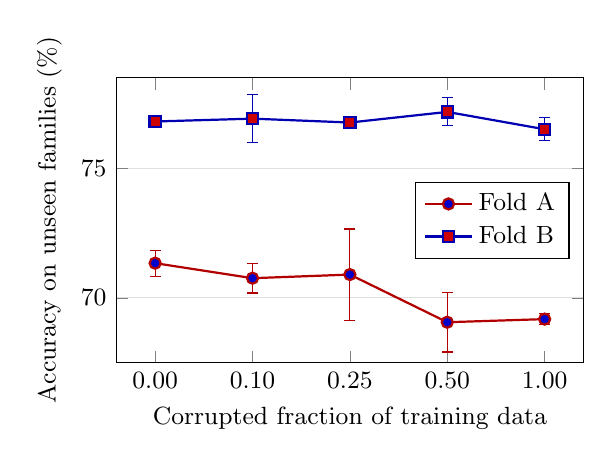
\begin{tikzpicture}
\begin{axis}[
  width=0.62\linewidth, height=5.2cm,
  xlabel={Corrupted fraction of training data},
  ylabel={Accuracy on unseen families (\%)},
  xtick={1,2,3,4,5},
  xticklabels={0.00,0.10,0.25,0.50,1.00},
  xmin=0.6, xmax=5.4,
  ymin=67.5, ymax=78.5,
  ymajorgrids=true, grid style={gray!25},
  legend cell align=left, legend style={font=\small, at={(0.97,0.5)}, anchor=east},
  tick label style={font=\small}, label style={font=\small},
  every axis plot/.append style={thick},
]
\addplot+[mark=*, color=red!70!black, error bars/.cd, y dir=both, y explicit]
  coordinates {(1,71.34) +- (0,0.50) (2,70.76) +- (0,0.57) (3,70.90) +- (0,1.76) (4,69.06) +- (0,1.15) (5,69.18) +- (0,0.21)};
\addlegendentry{Fold A}
\addplot+[mark=square*, color=blue!70!black, error bars/.cd, y dir=both, y explicit]
  coordinates {(1,76.81) +- (0,0.23) (2,76.92) +- (0,0.93) (3,76.77) +- (0,0.20) (4,77.18) +- (0,0.54) (5,76.51) +- (0,0.44)};
\addlegendentry{Fold B}
\end{axis}
\end{tikzpicture}
\caption{Mixed-3 accuracy on the fold's unseen families as the corrupted fraction grows at a fixed dataset size of 4{,}000 (0.00 is the clean baseline). Points are means over 3 seeds and error bars are $\pm$1 SD. The sweep is descriptive and was not tested inferentially.}
\label{fig:sweep}
\end{figure}

If diversity does not help, perhaps more corrupted data does. \Cref{fig:sweep} shows that it does not. In fold B, unseen-family accuracy stays within 0.7\ppts{} of the clean baseline at every corrupted fraction from 10\% to 100\%. In fold A it declines, with accuracy at 50\% and 100\% corruption about 2\ppts{} below the clean baseline, consistent with the secondary contrasts.

\subsection{Robustness does not transfer between families}
\label{sec:transfer}

\begin{table}[t]
\centering
\small
\caption{Transfer matrix: accuracy of each single-family model minus the clean baseline, in percentage points, averaged over seeds. Diagonal (bold): tested on the training family. Shading: red for losses and blue for gains, darker for larger magnitudes. Descriptive only.}
\label{tab:transfer}
\begin{tabular}{@{}l *{6}{c}@{}}
\toprule
Trained on $\downarrow$ / tested on $\rightarrow$ & \pfam{typo} & \pfam{formatting} & \pfam{deletion} & \pfam{shuffle} & \pfam{distractor} & \pfam{synonym} \\
\midrule
\pfam{typo}       & \negA$\mathbf{-0.7}$ & \negA$-0.9$ & \negA$-1.3$ & \negA$-0.8$ & \negB$-2.1$ & \negB$-1.9$ \\
\pfam{formatting} & $+0.1$ & $\mathbf{+0.3}$ & \posA$+0.5$ & $-0.3$ & \negC$-2.6$ & \negA$-0.9$ \\
\pfam{deletion}   & $-0.2$ & \negA$-0.5$ & \negA$\mathbf{-0.5}$ & \negA$-1.2$ & \negC$-2.6$ & \negB$-1.8$ \\
\pfam{shuffle}    & $+0.2$ & \negA$-1.1$ & $-0.2$ & $\mathbf{-0.3}$ & \negA$-1.4$ & \negA$-0.6$ \\
\pfam{distractor} & $-0.4$ & $+0.3$ & \posA$+0.6$ & \negA$-1.3$ & \posC$\mathbf{+18.1}$ & $-0.1$ \\
\pfam{synonym}    & $+0.0$ & $-0.1$ & $+0.3$ & \negA$-1.0$ & \posA$+1.4$ & \posA$\mathbf{+0.8}$ \\
\bottomrule
\end{tabular}
\end{table}

\Cref{tab:transfer} explains both findings. Five of the six families barely hurt a clean-trained model: it loses at most 3.7\ppts{} on them relative to its 78.8\% clean accuracy, and training on the family itself changes accuracy on that family by less than 1\ppts{}. With so little headroom, no training mixture can show much transfer. The exception is \pfam{distractor}. It costs the clean model 18\ppts{}, and training on it recovers the full loss ($+18.1$\ppts{}). No other family transfers to it: the off-diagonal entries in its column range from $-2.6$ to $+1.4$\ppts{}. A mixture therefore has nothing to transfer. Each family's robustness comes only from that family's own data.

\subsection{Exploratory: the distractor gap is an answer bias}
\label{sec:distractor}

This analysis was not pre-specified. \Cref{tab:bias} splits accuracy on the \pfam{distractor} test set by gold label. The untuned model answers ``Yes'' to only 0.8\% of questions with an appended distractor sentence, compared with 37.1\% on clean questions. Its \pfam{distractor} accuracy (37.4\%) therefore roughly equals the share of ``No'' items. Clean fine-tuning reduces this bias but does not remove it: the clean model's ``Yes'' rate falls from 64.7\% on clean questions to 38.8\% with a distractor, against a gold rate of 63.4\%. The high seed variance on this family reflects variation in the size of that shift. Fold A's Mixed-3, which never sees the family, shifts even further (31.1\% ``Yes''). Any model that saw \pfam{distractor} examples in training, including fold B's Mixed-3 with only 667 of them, answers ``Yes'' at the same rate as on clean input. Read this way, the largest robustness gap in our study is a perturbation-specific shift in the answer prior that a few hundred in-family examples correct, rather than a general failure to understand perturbed text.

\begin{table}[t]
\centering
\small
\caption{Exploratory answer-bias diagnostic on the clean and \pfam{distractor} test sets (mean $\pm$ SD over seeds; the untuned model has a single run). The gold ``Yes'' rate is 63.4\%.}
\label{tab:bias}
\begin{tabular}{@{}llcccc@{}}
\toprule
Condition & Test set & Predicted ``Yes'' & Acc.\ on gold ``Yes'' & Acc.\ on gold ``No'' & Accuracy \\
\midrule
\multirow{2}{*}{untuned} & clean & 37.1 & 48.1 & 82.0 & 60.5 \\
 & distractor & 0.8 & 1.3 & 100.0 & 37.4 \\
\multirow{2}{*}{clean} & clean & 64.7 $\pm$ 0.8 & 84.3 $\pm$ 0.5 & 69.3 $\pm$ 1.9 & 78.8 $\pm$ 0.7 \\
 & distractor & 38.8 $\pm$ 6.6 & 49.7 $\pm$ 7.2 & 80.1 $\pm$ 6.5 & 60.8 $\pm$ 3.2 \\
\multirow{2}{*}{NEFTune} & clean & 65.9 $\pm$ 3.4 & 86.0 $\pm$ 2.4 & 68.9 $\pm$ 4.9 & 79.7 $\pm$ 0.3 \\
 & distractor & 35.0 $\pm$ 7.0 & 46.5 $\pm$ 8.1 & 84.9 $\pm$ 5.3 & 60.5 $\pm$ 3.4 \\
\multirow{2}{*}{A: Mixed-3} & clean & 64.4 $\pm$ 2.2 & 83.6 $\pm$ 1.8 & 68.9 $\pm$ 2.8 & 78.2 $\pm$ 0.5 \\
 & distractor & 31.1 $\pm$ 6.7 & 41.0 $\pm$ 7.7 & 86.2 $\pm$ 5.6 & 57.5 $\pm$ 3.2 \\
\multirow{2}{*}{B: Mixed-3} & clean & 64.9 $\pm$ 1.7 & 85.0 $\pm$ 1.3 & 69.9 $\pm$ 2.6 & 79.5 $\pm$ 0.7 \\
 & distractor & 65.1 $\pm$ 1.7 & 84.8 $\pm$ 1.1 & 69.1 $\pm$ 3.0 & 79.1 $\pm$ 0.8 \\
\multirow{2}{*}{B: single \pfam{distractor}} & clean & 65.0 $\pm$ 1.1 & 84.3 $\pm$ 0.9 & 68.3 $\pm$ 1.7 & 78.4 $\pm$ 0.3 \\
 & distractor & 65.3 $\pm$ 1.3 & 84.9 $\pm$ 1.4 & 68.6 $\pm$ 1.7 & 78.9 $\pm$ 0.8 \\
\bottomrule
\end{tabular}
\end{table}

\section{Discussion}
\label{sec:discussion}

\paragraph{Why diversity did not help.} A mixture can only beat its components on unseen families if training on some perturbations gives robustness to others. \Cref{tab:transfer} shows almost no such transfer, so there is nothing for diversity to combine. This agrees with the vision finding that robustness rarely transfers between perturbation types \citep{kang2019transfer}, and it suggests that the ``diverse noise as insurance'' heuristic should not be assumed for small language models. Diversity is not harmful on the families it covers, though. Fold A's Mixed-3 matches the single-family models on seen families, and fold B's Mixed-3 is as robust to \pfam{distractor} as the dedicated single-family model despite seeing a third as many examples. A mixture is therefore a reasonable way to cover \emph{known} perturbation types. It just does not extend to unknown ones.

\paragraph{Perturbed training is not free.} In fold A, training on surface and deletion noise left the model somewhat less robust to unseen perturbations than clean training did, and \cref{tab:bias} shows that on \pfam{distractor} this goes together with a stronger shift towards ``No''. We do not have a mechanism for this, and the effect does not appear in fold B. However, it argues against adding perturbed data ``just in case'' without measuring its effect on the perturbations one actually cares about.

\paragraph{Practical implications.} At this scale, the most effective robustness intervention was to include the specific perturbation a deployment is expected to face. A few hundred examples were enough for the one family with a large gap. Robustness evaluations should also check answer-bias statistics: a large accuracy drop can come from a shift in the answer prior rather than from a failure of comprehension.

\section{Limitations}
\label{sec:limitations}

\begin{itemize}
  \item \textbf{Scale and scope.} One model (0.5B parameters), one task (BoolQ), and three seeds. The optional 1.5B scale check in our protocol was not run. Larger models may transfer robustness more readily: \citet{alajrami2025noisy} report more consistent gains from noisy tuning for 70B-scale models.
  \item \textbf{Asymmetric folds.} Fold A's unseen set contains \pfam{distractor}, the one hard and high-variance family (seed SD up to 5.3\ppts{}), while fold B's unseen families are nearly solved by clean training. Fold B therefore had little headroom to show any effect.
  \item \textbf{Mild perturbations.} Five families cost a clean-trained model at most 3.7\ppts{}, which limits statistical power for any diversity contrast on them. Stronger perturbations might give a different answer.
  \item \textbf{Perturbation design.} Perturbations touch only the question. \pfam{synonym} replacement with WordNet is only approximately meaning-preserving (``soil'' becomes ``dirty'' in \cref{tab:families}). \pfam{distractor} draws from a pool of 8 sentences shared by its training and test versions, so the in-family gain in \cref{tab:transfer} may partly reflect familiarity with those sentences. The out-of-family results are not affected, because the family is unseen there.
  \item \textbf{Statistics.} The bootstrap interval captures test-item uncertainty only. Training randomness enters through the seed-SD criterion, which with three seeds is itself imprecise. Secondary contrasts are uncorrected for multiplicity, and \cref{sec:distractor} is exploratory.
\end{itemize}

\section{Conclusion}

At a fixed corruption volume, fine-tuning Qwen2.5-0.5B-Instruct on a mixture of three perturbation families did not make it more robust to unseen families than training on a single family, and neither did a larger corrupted fraction. Robustness from noisy fine-tuning was specific to the family trained on. The one perturbation that caused a large drop did so mainly by shifting the answer prior, and only data containing it fixed the problem. If a model must be robust to a particular kind of noise, our results suggest including that noise in training rather than relying on diversity to reach it.

\section*{Reproducibility Statement}

All code, the data-generation pipeline (with SHA-256 manifests of every training file), per-run configurations, step-level training logs, metrics, and per-item test predictions for all 55 runs are available at \url{https://github.com/SoumyaranjanPanda01/noise-diversity-research}. The protocol, every deviation from it, and a laboratory log are in the repository's \texttt{docs/} folder. Every number in this paper is produced by \texttt{scripts/analyze.py} and \texttt{scripts/diag\_distractor.py} from the released run records.

\begin{thebibliography}{99}

\bibitem[Agrawal et al.(2025)]{agrawal2025enhancing}
Aryan Agrawal, Lisa Alazraki, Shahin Honarvar, and Marek Rei.
\newblock Enhancing {LLM} robustness to perturbed instructions: An empirical study.
\newblock In \emph{ICLR 2025 Workshop on Building Trust in Language Models and Applications}, 2025.
\newblock arXiv:2504.02733.

\bibitem[Alajrami et al.(2025)]{alajrami2025noisy}
Ahmed Alajrami, Xingwei Tan, and Nikolaos Aletras.
\newblock Fine-tuning on noisy instructions: Effects on generalization and performance.
\newblock In \emph{Proceedings of AACL}, 2025.
\newblock arXiv:2510.03528.

\bibitem[Belinkov and Bisk(2018)]{belinkov2018synthetic}
Yonatan Belinkov and Yonatan Bisk.
\newblock Synthetic and natural noise both break neural machine translation.
\newblock In \emph{International Conference on Learning Representations}, 2018.
\newblock arXiv:1711.02173.

\bibitem[Clark et al.(2019)]{clark2019boolq}
Christopher Clark, Kenton Lee, Ming-Wei Chang, Tom Kwiatkowski, Michael Collins, and Kristina Toutanova.
\newblock {BoolQ}: Exploring the surprising difficulty of natural yes/no questions.
\newblock In \emph{Proceedings of NAACL-HLT}, 2019.
\newblock arXiv:1905.10044.

\bibitem[Efron and Tibshirani(1993)]{efron1993bootstrap}
Bradley Efron and Robert J. Tibshirani.
\newblock \emph{An Introduction to the Bootstrap}.
\newblock Chapman \& Hall, 1993.

\bibitem[Hendrycks and Dietterich(2019)]{hendrycks2019benchmarking}
Dan Hendrycks and Thomas Dietterich.
\newblock Benchmarking neural network robustness to common corruptions and perturbations.
\newblock In \emph{International Conference on Learning Representations}, 2019.
\newblock arXiv:1903.12261.

\bibitem[Hendrycks et al.(2020)]{hendrycks2020augmix}
Dan Hendrycks, Norman Mu, Ekin D. Cubuk, Barret Zoph, Justin Gilmer, and Balaji Lakshminarayanan.
\newblock {AugMix}: A simple data processing method to improve robustness and uncertainty.
\newblock In \emph{International Conference on Learning Representations}, 2020.
\newblock arXiv:1912.02781.

\bibitem[Hu et al.(2022)]{hu2022lora}
Edward J. Hu, Yelong Shen, Phillip Wallis, Zeyuan Allen-Zhu, Yuanzhi Li, Shean Wang, Lu Wang, and Weizhu Chen.
\newblock {LoRA}: Low-rank adaptation of large language models.
\newblock In \emph{International Conference on Learning Representations}, 2022.
\newblock arXiv:2106.09685.

\bibitem[Jain et al.(2024)]{jain2024neftune}
Neel Jain, Ping-yeh Chiang, Yuxin Wen, John Kirchenbauer, Hong-Min Chu, Gowthami Somepalli, Brian R. Bartoldson, Bhavya Kailkhura, Avi Schwarzschild, Aniruddha Saha, Micah Goldblum, Jonas Geiping, and Tom Goldstein.
\newblock {NEFTune}: Noisy embeddings improve instruction finetuning.
\newblock In \emph{International Conference on Learning Representations}, 2024.
\newblock arXiv:2310.05914.

\bibitem[Kang et al.(2019)]{kang2019transfer}
Daniel Kang, Yi Sun, Tom Brown, Dan Hendrycks, and Jacob Steinhardt.
\newblock Transfer of adversarial robustness between perturbation types.
\newblock \emph{arXiv preprint arXiv:1905.01034}, 2019.

\bibitem[Li and Sen(2026)]{li2026analyzing}
Lingfang Li and Procheta Sen.
\newblock Analyzing the effect of noise in {LLM} fine-tuning.
\newblock \emph{arXiv preprint arXiv:2604.12469}, 2026.

\bibitem[Miller(1995)]{miller1995wordnet}
George A. Miller.
\newblock {WordNet}: A lexical database for {English}.
\newblock \emph{Communications of the ACM}, 38(11):39--41, 1995.

\bibitem[Qwen Team(2025)]{qwen2025qwen25}
Qwen Team.
\newblock {Qwen2.5} technical report.
\newblock \emph{arXiv preprint arXiv:2412.15115}, 2025.

\bibitem[Tram{\`e}r and Boneh(2019)]{tramer2019adversarial}
Florian Tram{\`e}r and Dan Boneh.
\newblock Adversarial training and robustness for multiple perturbations.
\newblock In \emph{Advances in Neural Information Processing Systems}, 2019.
\newblock arXiv:1904.13000.

\bibitem[Wei and Zou(2019)]{wei2019eda}
Jason Wei and Kai Zou.
\newblock {EDA}: Easy data augmentation techniques for boosting performance on text classification tasks.
\newblock In \emph{Proceedings of EMNLP-IJCNLP}, 2019.
\newblock arXiv:1901.11196.

\bibitem[Zhang et al.(2024)]{zhang2024raft}
Tianjun Zhang, Shishir G. Patil, Naman Jain, Sheng Shen, Matei Zaharia, Ion Stoica, and Joseph E. Gonzalez.
\newblock {RAFT}: Adapting language model to domain specific {RAG}.
\newblock In \emph{Conference on Language Modeling}, 2024.
\newblock arXiv:2403.10131.

\end{thebibliography}

\appendix

\section{Implementation Details}
\label{app:details}

\begin{table}[h]
\centering
\small
\caption{Hyperparameters, identical for every condition.}
\label{tab:hparams}
\begin{tabular}{@{}ll@{}}
\toprule
Base model & Qwen2.5-0.5B-Instruct \\
LoRA rank / $\alpha$ / dropout & 16 / 32 / 0.05 \\
LoRA target modules & \texttt{q,k,v,o,gate,up,down} projections \\
Trainable parameters & 8{,}798{,}208 of 502{,}830{,}976 (1.75\%) \\
Optimizer & AdamW, learning rate $2\times10^{-4}$, weight decay 0 \\
Schedule & cosine decay, 3\% linear warmup \\
Gradient clipping & 1.0 \\
Epochs / optimizer steps & 2 / 500 \\
Effective batch size & 16 (micro-batch 4, gradient accumulation 4) \\
Maximum sequence length & 512 tokens (passage truncated if needed) \\
Loss & answer token and end-of-turn token only \\
Precision & fp16 autocast with fp32 master weights \\
NEFTune $\alpha$ (NEFTune condition only) & 5 \\
Seeds & 0, 1, 2 \\
Hardware & 1 $\times$ NVIDIA T4 (16 GB) \\
\bottomrule
\end{tabular}
\end{table}

The system prompt is: \emph{``You are a helpful assistant. Read the passage and answer the question with only `Yes' or `No'.''} The user turn contains the passage and the question. The validation set is evaluated after each epoch for monitoring only. The development set was not used, because no tuning was done. With micro-batch 4 and gradient accumulation 4, the loss is normalised by the number of target tokens in the full batch of 16, so the accumulated gradient equals the full-batch gradient.

\section{Protocol Deviations}
\label{app:deviations}

All of the following were logged before any test-set result was seen.

\begin{enumerate}
  \item[D1] The NEFTune baseline is a single condition shared across folds rather than one per fold, because NEFTune on clean data does not depend on the fold. The study has 54 training runs instead of 57.
  \item[D2] The EDA baseline uses only operations that do not correspond to the fold's unseen families (standard EDA includes synonym, swap, and deletion edits, which would break the family holdout). Random insertion copies a word already in the question. One operation per example, with $\alpha{=}0.1$.
  \item[D3] A non-determinism bug in synonym selection (iteration order of a Python set) was fixed and the affected files regenerated, before any model was trained on them.
  \item[D4] Evaluation compares the ``Yes'' and ``No'' next-token logits instead of parsing generated text, applied identically to all models including the untuned one.
  \item[D5] The loss is computed on answer tokens only, and passages (never questions) are truncated to fit 512 tokens.
  \item[D6] Training ran on a cloud T4 GPU with mixed precision, because the development machine has no GPU.
\end{enumerate}

\section{Full Results}
\label{app:full}

\begin{table}[h]
\centering
\scriptsize
\setlength{\tabcolsep}{3pt}
\caption{Test accuracy (\%) for every condition and test version, mean $\pm$ SD over 3 seeds (the untuned model has a single run). ``Seen'' and ``unseen'' average the fold's three seen or unseen families.}
\label{tab:full}
\begin{tabular}{@{}l *{9}{c}@{}}
\toprule
Condition & clean & \pfam{typo} & \pfam{formatting} & \pfam{deletion} & \pfam{shuffle} & \pfam{distractor} & \pfam{synonym} & seen & unseen \\
\midrule
untuned & 60.5 & 55.9 & 56.3 & 59.9 & 59.5 & 37.4 & 50.0 & -- & -- \\
clean & 78.8$\pm$0.7 & 77.6$\pm$0.6 & 77.3$\pm$0.5 & 75.5$\pm$0.1 & 78.1$\pm$1.3 & 60.8$\pm$3.2 & 75.1$\pm$1.1 & -- & -- \\
NEFTune & 79.7$\pm$0.3 & 78.1$\pm$0.2 & 77.7$\pm$0.9 & 75.5$\pm$0.6 & 77.9$\pm$0.4 & 60.5$\pm$3.4 & 74.9$\pm$0.9 & -- & -- \\
\midrule
\multicolumn{10}{@{}l}{\emph{Fold A} (seen: \pfam{typo}, \pfam{formatting}, \pfam{deletion})} \\
single \pfam{typo} & 78.4$\pm$1.0 & 76.9$\pm$0.6 & 76.5$\pm$0.7 & 74.1$\pm$1.0 & 77.3$\pm$0.8 & 58.7$\pm$2.2 & 73.2$\pm$1.1 & 75.8$\pm$0.6 & 69.7$\pm$0.3 \\
single \pfam{formatting} & 80.0$\pm$0.6 & 77.8$\pm$0.6 & 77.7$\pm$0.7 & 75.9$\pm$0.4 & 77.8$\pm$0.2 & 58.2$\pm$5.3 & 74.2$\pm$0.8 & 77.1$\pm$0.2 & 70.1$\pm$1.6 \\
single \pfam{deletion} & 78.6$\pm$0.9 & 77.4$\pm$0.7 & 76.9$\pm$0.4 & 74.9$\pm$0.4 & 77.0$\pm$0.2 & 58.2$\pm$1.4 & 73.3$\pm$0.2 & 76.4$\pm$0.3 & 69.5$\pm$0.4 \\
Mixed-3, 0.50 & 78.2$\pm$0.5 & 76.6$\pm$1.0 & 77.1$\pm$0.9 & 74.7$\pm$0.6 & 76.3$\pm$1.0 & 57.5$\pm$3.2 & 73.3$\pm$0.8 & 76.1$\pm$0.8 & 69.1$\pm$1.2 \\
Mixed-3, 0.10 & 78.9$\pm$0.8 & 77.6$\pm$0.7 & 76.7$\pm$0.5 & 75.2$\pm$0.3 & 77.5$\pm$0.8 & 60.1$\pm$2.6 & 74.7$\pm$1.0 & 76.5$\pm$0.3 & 70.8$\pm$0.6 \\
Mixed-3, 0.25 & 78.9$\pm$1.0 & 77.1$\pm$0.6 & 76.7$\pm$0.7 & 75.3$\pm$0.6 & 77.8$\pm$1.0 & 60.9$\pm$3.6 & 74.0$\pm$1.0 & 76.4$\pm$0.4 & 70.9$\pm$1.8 \\
Mixed-3, 1.00 & 78.0$\pm$0.6 & 77.3$\pm$0.9 & 77.3$\pm$1.4 & 74.5$\pm$0.6 & 76.5$\pm$0.5 & 57.2$\pm$1.2 & 73.9$\pm$0.3 & 76.4$\pm$0.8 & 69.2$\pm$0.2 \\
EDA augment & 79.4$\pm$0.8 & 78.2$\pm$0.3 & 77.6$\pm$0.7 & 75.0$\pm$1.1 & 77.5$\pm$0.7 & 59.0$\pm$2.9 & 74.4$\pm$0.3 & 76.9$\pm$0.7 & 70.3$\pm$0.7 \\
\midrule
\multicolumn{10}{@{}l}{\emph{Fold B} (seen: \pfam{shuffle}, \pfam{distractor}, \pfam{synonym})} \\
single \pfam{shuffle} & 78.5$\pm$0.4 & 77.8$\pm$0.5 & 76.2$\pm$0.9 & 75.2$\pm$0.4 & 77.8$\pm$0.3 & 59.4$\pm$1.4 & 74.5$\pm$0.2 & 70.6$\pm$0.4 & 76.4$\pm$0.3 \\
single \pfam{distractor} & 78.4$\pm$0.3 & 77.2$\pm$0.6 & 77.6$\pm$0.5 & 76.1$\pm$0.5 & 76.9$\pm$1.1 & 78.9$\pm$0.8 & 75.0$\pm$0.3 & 76.9$\pm$0.6 & 77.0$\pm$0.2 \\
single \pfam{synonym} & 79.1$\pm$0.4 & 77.6$\pm$0.7 & 77.2$\pm$0.2 & 75.7$\pm$0.8 & 77.1$\pm$0.8 & 62.2$\pm$1.3 & 75.9$\pm$0.2 & 71.8$\pm$0.2 & 76.9$\pm$0.4 \\
Mixed-3, 0.50 & 79.5$\pm$0.7 & 78.2$\pm$1.0 & 77.4$\pm$0.4 & 75.9$\pm$0.9 & 77.7$\pm$1.4 & 79.1$\pm$0.8 & 76.0$\pm$0.4 & 77.6$\pm$0.8 & 77.2$\pm$0.5 \\
Mixed-3, 0.10 & 78.9$\pm$0.8 & 78.1$\pm$1.0 & 77.6$\pm$1.1 & 75.1$\pm$1.2 & 77.5$\pm$0.5 & 77.6$\pm$0.3 & 75.2$\pm$0.2 & 76.7$\pm$0.2 & 76.9$\pm$0.9 \\
Mixed-3, 0.25 & 79.0$\pm$0.5 & 77.1$\pm$0.7 & 78.1$\pm$0.6 & 75.2$\pm$0.5 & 77.9$\pm$0.5 & 78.9$\pm$0.7 & 75.0$\pm$0.3 & 77.3$\pm$0.4 & 76.8$\pm$0.2 \\
Mixed-3, 1.00 & 78.9$\pm$0.5 & 77.0$\pm$0.8 & 77.2$\pm$0.6 & 75.3$\pm$0.2 & 77.2$\pm$0.1 & 78.5$\pm$0.5 & 75.6$\pm$0.9 & 77.1$\pm$0.3 & 76.5$\pm$0.4 \\
EDA augment & 79.7$\pm$0.7 & 78.3$\pm$0.2 & 77.6$\pm$0.2 & 76.6$\pm$0.3 & 78.0$\pm$0.7 & 61.8$\pm$4.1 & 76.9$\pm$0.4 & 72.3$\pm$1.3 & 77.5$\pm$0.1 \\
\bottomrule
\end{tabular}
\end{table}

\end{document}
\typeout{get arXiv to do 4 passes: Label(s) may have changed. Rerun}
